\section{Digital Twin of the Smart Grapple}
\label{sec:sim}
Due to the scarce availability of sea trials, the \gls{usg} is mostly tested in the lab. Additionally, a simulation-based, digital twin approach is used to validate the system between field tests.

Simulation is conducted using the \gls{marus} tool. The source code of the \gls{usg} is stored in a separate Docker container from the \gls{marus} interface. This \gls{sil} method helps to bridge the sim-to-real gap by allowing the same source code to run in the real system with minimal changes. It also accelerates development since no extra code is needed for simulation.

\textbf{Scope of the Simulation.}
The digital twin is currently able to reproduce navigation of the \gls{usg}. That means the perception, planning, and tracking sub-modules are already integrated in the simulation pipeline. Figure~\ref{fig:simPipe} visualizes the software stack for simulation and Figure~\ref{fig:simGameView} shows the digital twin in the virtual environment. 

\begin{figure}[ht]
	\centering
	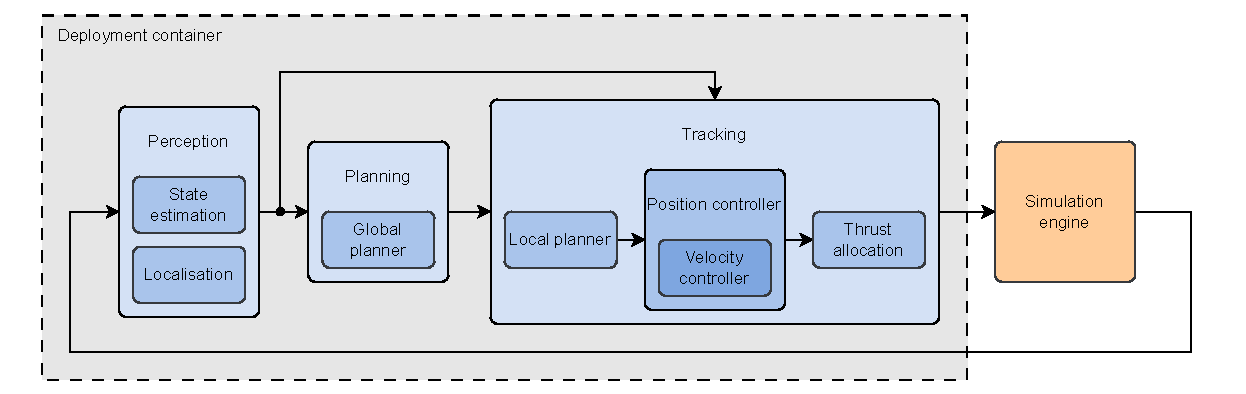
\includegraphics[width=\textwidth]{img/tracking_software_stack.drawio.pdf}
	\caption{Software stack of the simulation pipeline}
	\label{fig:simPipe}
\end{figure}

\textbf{MARUS Engine.}
The \gls{marus} simulation engine was developed by the \textit{Laboratory for Underwater Systems and Technologies} at the University of Zagreb \cite{9976969}. It is an open-source simulator for marine robotics based on the Unity3D software. The main benefits of this simulator are:
\begin{itemize}
    \item Native ROS 2 support,
    \item Realistic underwater visual data (needed for machine learning computer vision algorithms),
    \item Availability of standard sensors in marine robotics, such as \gls{dvl}, depth sensor, sonar, and acoustic communication,
    \item Mesh-based approximation of hydrodynamics,
    \item Ongoing development.
\end{itemize}

\begin{figure}[ht]
	\centering
	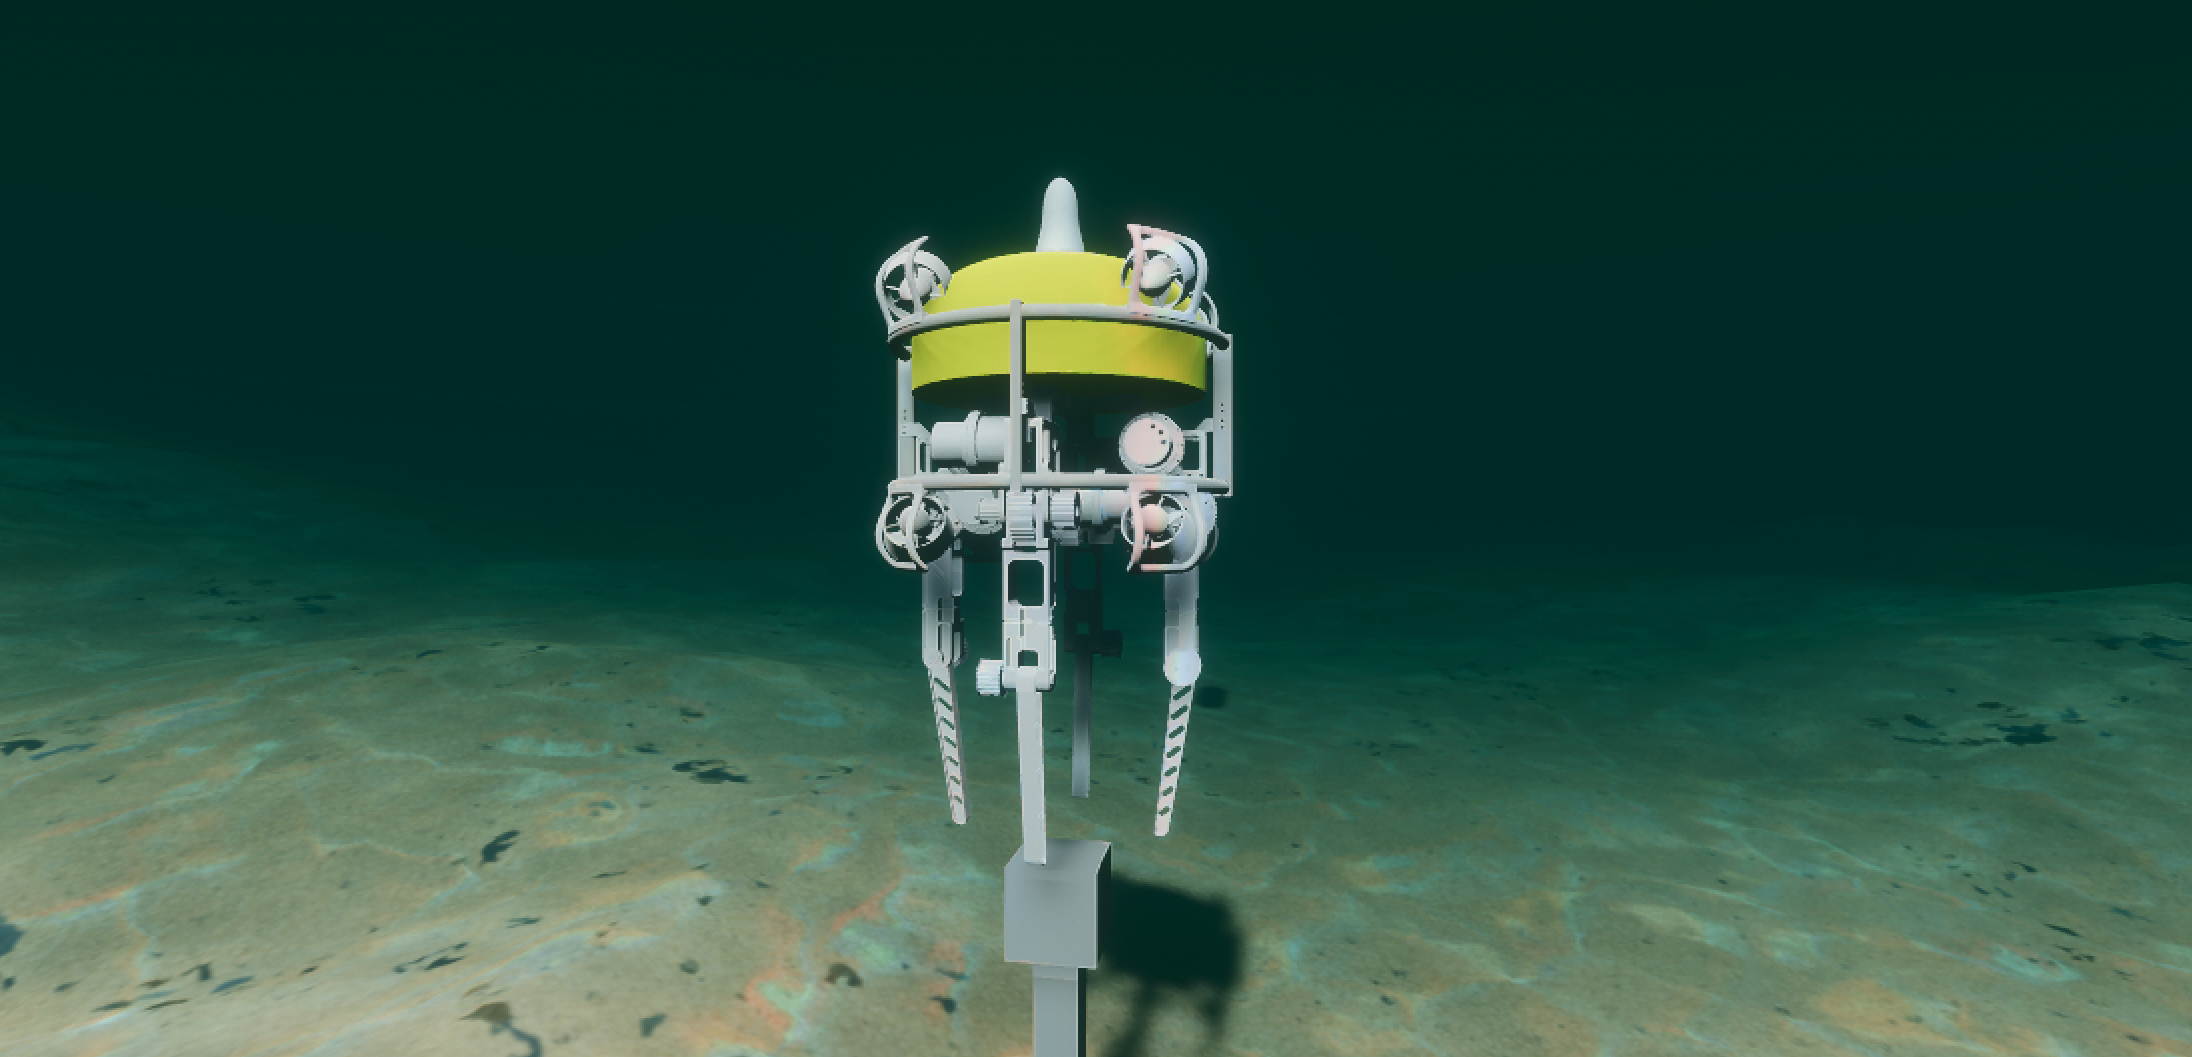
\includegraphics[width=\textwidth]{img/unity_sim_game_view.png}
	\caption{Digital twin in the virtual environment}
	\label{fig:simGameView}
\end{figure}